\section{INTRODUCTION}\label{Sec:intro}
%{\color{red}\textbf{Introduction:}}\cite{javaid2020robotics}
%
%\begin{itemize}
%    \item What is the motivation for investigating this area.
%    \item Why other people have not solved it.
%    \item Define the problem and current issues.
%    \item What is the need?
%    \item If solving this problem who will benefit?
%    \item How do you propose to solve the problem?
%    \item How do you propose to evaluate the solution?
%    \item Outline the paper.
%\end{itemize}

The pandemic COVID-19 raises people's attention to robot applications. The outbreak of the disease makes the medical personnel unsatisfied for handling the heavy treatment. Also, because the virus is highly transmissible, many doctors and nurses encounter the risk of being infected. Under this circumstance, robots play a variety of roles in the medical field, which help to assist related works as well as reduce the unnecessary contact between patients and medical personnel. To prevent infection of COVID-19, disinfection is an essential approach. Currently, most of the disinfection works in hospitals rely on humans by hand, which is a waste of manpower especially in such circumstances which are in great need. Also, disinfection by humans increases the chances of contact between the virus and healthy people, which speeds up the spread of COVID-19. Therefore, an automatic robot that is able to complete the disinfection task of precise fixed-point and complete coverage alcohol spraying, as well as UV sterilization meanwhile is important and useful. This robot allows medical personnel to work on other more complex tasks and reduce their workloads. However, the research on this kind of robot still needs to be improved. First, the robot needs to detect a nearby environment to adjust the mode of spraying alcohol to maximize efficiency. Second, the robot arm should be highly flexible in order to disinfect the specific object with full coverage. Third, the robot is required to has the capability to automatically back to the charge station with a low battery, which is detected by the robot itself.
\par In this paper we first propose a robot system that integrates designed functions and required hardware and software technology. Then, hypotheses and experiments to validate the feasibility and accuracy of the designed robot are put forward. Finally, we conclude the current proposal of the robot design and discuss potential applications and optimization.
% \begin{figure}[h!]
%   \centering
%   
\includegraphics[scale=1.7]{figures/universe.jpg}
%   \caption{The Universe}
%   \label{Fig:universe}
% \end{figure}

\subsection{Related Work}
Robots play an important part in medical service. The International Federation of Robotics (IFR) has four major classifications of medical robots, namely: rehabilitation robots, surgical robots, assistive robots and service robots. Common medical service robots include transportation service robots in medical places and disinfection service robots.
% \begin{figure}[htbp] 
% \centering 
% 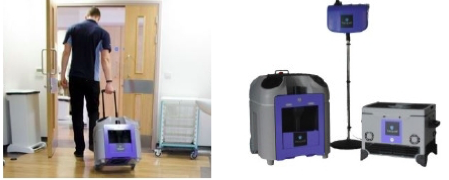
\includegraphics[width=0.4\textwidth]{figures/WechatIMG346.png} 
% \caption{Bioquell BQ-50} 
% \label{bq50} 
% \end{figure}
BQ-50 intelligent hydrogen peroxide gas generator launched by the British company Bioquell has been scientifically certified to provide solutions for air and surface pollution. It realizes one-key automatic sterilization operation\cite{rowan2020unlocking}. This product is mainly used in few wards of hospitals. The equipment is connected to the console, and the entire sterilization process can be monitored through the two buttons on the console. 
% \begin{figure}[h] 
% \centering 
% 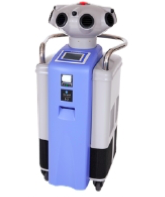
\includegraphics[width=0.2\textwidth]{figures/WechatIMG347.png} 
% \caption{Bioquell Z2} 
% \label{z2} 
% \end{figure}
Bioqull’s latest generation product Bioquell Z2 uses hydrogen peroxide gas to effectively sterilize a certain range. The unique dual-loop technology can quickly and efficiently purify the indoor environment without the need for environmental protection. 
% \begin{figure}[h] 
% \centering 
% 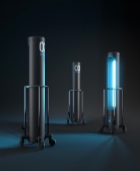
\includegraphics[width=0.2\textwidth]{figures/WechatIMG348.png} 
% \caption{Surfacide Helios} 
% \label{sh} 
% \end{figure}

    % \begin{figure}[htbp]
    % \centering
    % \begin{minipage}[t]{0.24\textwidth}
    % \centering
    % 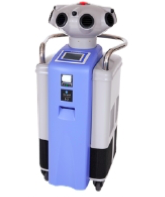
\includegraphics[width=3cm]{figures/WechatIMG347.png}
    % \caption{Bioquell Z2}
    % \label{z2}
    % \end{minipage}
    % \begin{minipage}[t]{0.24\textwidth}
    % \centering
    % 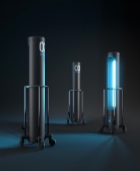
\includegraphics[width=3cm]{figures/WechatIMG348.png}
    % \caption{Surfacide Helios}
    % \label{sh}
    % \end{minipage}
    % \end{figure}

 
Surfacide UV disinfection system, developed by a UK company, has changed the previous single application mode of UV disinfection technology in the healthcare sector\cite{bedell_buchaklian_perlman_2016}. By implementing multiple light emitters in the hospital environment, it overcomes the inherent problems of incomplete disinfection caused by the use of a single UV emitter system that is easily restricted by conditions such as shadows and distance.


In general, according to the current research, ultraviolet disinfection still needs to be work in an unmanned environment but no sufficient research on the coverage of disinfection currently. Therefore, this article focus on the precise fixed point and complete coverage of alcohol spray and disinfection tasks. Meanwhile, the use of alcohol disinfection ensures that the robot disinfection and the staff perform work at the same time.
